\documentclass[crop,tikz]{standalone}

\usepackage{libertinus}
\usepackage{libertinust1math}
\usepackage[T1]{fontenc}
\usepackage[scaled=0.79]{beramono}

\usetikzlibrary{positioning}
\usetikzlibrary{calc}

\begin{document}

\newlength\hdist\setlength\hdist{24mm}
\newlength\vdist\setlength\vdist{8mm}

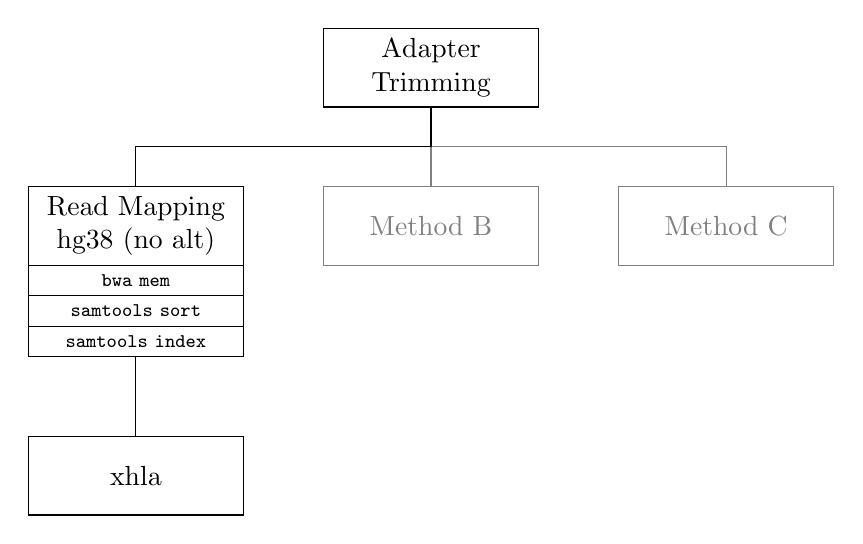
\begin{tikzpicture}[
    main/.style={
        draw,
        text width=25mm,
        align=center,
        minimum height=10mm,
    },
    minor/.style={
        main,
        minimum height=0mm,
        font=\ttfamily\scriptsize,
    }
    ]
    \node [main] (xhlaMap) { Read Mapping\\hg38 (no alt)};
    \node [minor, below=-\pgflinewidth of xhlaMap] (xhlaMap1) {bwa mem};
    \node [minor, below=-\pgflinewidth of xhlaMap1] (xhlaMap2) {samtools sort};
    \node [minor, below=-\pgflinewidth of xhlaMap2] (xhlaMap3) {samtools index};

    \node [main, below=\vdist of xhlaMap3] (xhla) {xhla};
    \draw (xhlaMap3) -- (xhla);

    \node [main,gray,right=\hdist of xhlaMap] (methodB) {Method B};
    \node [main,gray,right=\hdist of methodB] (methodC) {Method C};

    \node [main, anchor=south] (trim) at ($(xhlaMap.north west)!.5!(methodC.north east) + (0,\vdist)$) {Adapter Trimming};

    \draw[gray] (trim.south) -- +(0,-.5\vdist) -| (methodB.north);
    \draw[gray] (trim.south) -- +(0,-.5\vdist) -| (methodC.north);
    \draw (trim.south) -- +(0,-.5\vdist) -| (xhlaMap.north);
\end{tikzpicture}

\end{document}
